\documentclass[11pt]{article}

\usepackage[margin=1in]{geometry}
\usepackage{amsmath, amssymb}
\usepackage[utf8]{inputenc}
\usepackage[T1]{fontenc}
\usepackage{lmodern}
\usepackage{microtype}
\usepackage{graphicx}
\usepackage{booktabs}
\usepackage{array}
\usepackage{tabularx}
\usepackage{textcomp}
\usepackage{float}
\usepackage{xcolor}
\usepackage{fancyhdr}
\usepackage[font=small,labelfont=bf,skip=5pt]{caption}
\usepackage{listings}
\lstdefinestyle{pycode}{
  language=Python, basicstyle=\ttfamily\scriptsize,
  keywordstyle=\color{psink}\bfseries, commentstyle=\color{psaccent}\itshape,
  stringstyle=\color{psink}, numbers=left, numberstyle=\tiny\color{psrule},
  numbersep=7pt, breaklines=true, breakatwhitespace=true, showstringspaces=false,
  frame=none, xleftmargin=20pt, aboveskip=6pt, belowskip=6pt, columns=fullflexible,
  keepspaces=true, upquote=true,
}
\lstset{style=pycode}

\definecolor{psink}{RGB}{23,54,93}
\definecolor{psaccent}{RGB}{192,80,77}
\definecolor{psrule}{RGB}{200,209,222}

\usepackage[colorlinks=true,allcolors=psink]{hyperref}

\graphicspath{{./}}
\emergencystretch=3em

\setlength{\textfloatsep}{10pt plus 2pt minus 2pt}
\setlength{\intextsep}{10pt plus 2pt minus 2pt}
\setlength{\abovecaptionskip}{4pt}
\setlength{\belowcaptionskip}{0pt}

\makeatletter
\renewcommand\section{\@startsection{section}{1}{0pt}%
  {-2.6ex \@plus -1ex \@minus -.2ex}{1.3ex \@plus .2ex}%
  {\normalfont\scshape\large\color{psink}}}   % lmr has no bold small caps
\renewcommand\subsection{\@startsection{subsection}{2}{0pt}%
  {-2.2ex \@plus -1ex \@minus -.2ex}{1.0ex \@plus .2ex}%
  {\normalfont\bfseries\normalsize\color{psink}}}
\renewcommand\subsubsection{\@startsection{subsubsection}{3}{0pt}%
  {-1.9ex \@plus -.8ex \@minus -.2ex}{0.8ex \@plus .2ex}%
  {\normalfont\bfseries\itshape\normalsize\color{psink}}}
\renewcommand\subparagraph{\@startsection{subparagraph}{5}{0pt}%
  {-1.6ex \@plus -.6ex \@minus -.2ex}{0.5ex \@plus .1ex}%
  {\normalfont\itshape\normalsize\color{psink}}}
\renewcommand\paragraph{\@startsection{paragraph}{4}{0pt}%
  {1.7ex \@plus 1ex \@minus .2ex}{-0.9em}%
  {\normalfont\bfseries\normalsize\color{psink}}}
\makeatother

\newenvironment{tight}
  {\begin{itemize}\setlength{\itemsep}{3pt}\setlength{\parskip}{0pt}%
   \setlength{\topsep}{3pt}\setlength{\leftmargini}{1.4em}}
  {\end{itemize}}

\setcounter{secnumdepth}{0}   % headings carry the assignment's own labels
\setlength{\headheight}{22pt}
\pagestyle{fancy}
\fancyhf{}
\fancyhead[L]{\footnotesize\scshape\color{psink} MGT 595 \textemdash\ Problem Set 7}
\fancyhead[R]{\footnotesize\color{psink}\thepage}
\renewcommand{\headrulewidth}{0.4pt}
\renewcommand{\headrule}{\hbox to\headwidth{%
  \color{psrule}\leaders\hrule height \headrulewidth\hfill}}

\begin{document}

\thispagestyle{empty}
\begin{flushleft}
{\bfseries\LARGE\color{psink} Quantitative Investing}\\[3pt]
{\scshape\Large\color{psink} Problem Set 7}\\[10pt]
{\color{psrule}\rule{\textwidth}{1.2pt}}\\[5pt]
{\small Ashley Wen\,(xw564)\quad\textbar\quad Emily Wu\,(esw63)%
\quad\textbar\quad Grace Gu\,(xg325)\hfill \today}
\end{flushleft}

\vspace{1.4em}

{\color{psink}\textbf{Contents.}} Part I discusses what quality is and compares four ways of
measuring it (gross profitability, BAB, QMJ and RMW). Part II documents the flat security
market line in the 49 value-weighted industry portfolios. Parts III and IV run Fama--MacBeth
tests of the four-factor model augmented with BAB, QMJ, RMW and all three together. Part V
proposes a further test and evaluates an LLM-invented quality factor.

\vspace{0.8em}

% Problem Set 7 -- Part I. Converted verbatim from part I &V/PS7_PartI&V.docx.

\section{Part I: Conceptual}

\subsection*{Question 1}
Quality refers to firms with strong profitability, sustainable growth, and financial stability. These characteristics should affect stock valuations because they influence future cash flows and risk. Higher quality does not necessarily mean higher expected returns, since investors may already pay a premium for these firms, and safer firms may have lower required returns. It is surprising that high-quality stocks can earn higher risk-adjusted returns, potentially reflecting mispricing or risks not captured by traditional models.

\subsection*{Question 2}
Quality is commonly measured through profitability (gross or operating profits), growth (improvements in profitability), and safety (low leverage, stable earnings, and low default risk). There is no single obvious measure because quality is multidimensional, and each indicator captures only one aspect. A composite measure such as QMJ provides a broader assessment, but its choice of variables and weights introduces subjectivity.

\subsection*{Question 3}

\paragraph{Comparison of quality measures.}
Novy-Marx measures gross profitability (gross profits/assets), while Fama--French's RMW uses operating profitability relative to book equity, accounting for additional expenses. Both focus on profitability, whereas QMJ combines profitability, growth, and safety to capture broader firm quality. BAB differs by focusing on market beta and leverage constraints rather than fundamental quality.

\paragraph{Which measure is more reasonable?}
I find gross profitability appealing because it is simple and transparent. RMW captures more expenses but is sensitive to book equity. QMJ provides a broader measure but introduces more complexity and discretion. BAB is less convincing as a quality measure because low beta does not necessarily imply strong fundamentals.

\paragraph{Why might these measures predict returns?}
Gross profitability and RMW may predict returns because profitability helps forecast future earnings, which investors may underestimate. QMJ may outperform if investors underprice sustainable quality. BAB earns a premium because leverage-constrained investors favor high-beta stocks, flattening the security market line.

\paragraph{Are these explanations consistent with market efficiency?}
Risk compensation is consistent with market efficiency, while persistent mispricing challenges it. BAB can arise in a rational market with leverage constraints. Therefore, these return patterns do not necessarily imply market inefficiency.

\subsection*{AI integration: auditing the LLM on quality definitions}

\paragraph{Our one-sentence characterizations.}
\begin{tight}
  \item \textbf{Novy-Marx.} Quality is measured by gross profitability (revenue minus cost of goods sold, divided by total assets), capturing how efficiently a firm generates profits from its assets.
  \item \textbf{Frazzini and Pedersen.} BAB measures defensiveness through market beta rather than fundamental quality, exploiting leverage constraints by taking leveraged long positions in low-beta assets and short positions in high-beta assets.
  \item \textbf{Asness, Frazzini, and Pedersen.} QMJ defines quality through profitability, growth, and safety, combining these dimensions to construct a strategy that buys high-quality firms and shorts low-quality firms.
  \item \textbf{Fama and French.} RMW captures quality through operating profitability, constructing a factor that goes long firms with robust operating profitability and short firms with weak operating profitability.
\end{tight}

\paragraph{(i)}
The answer contains several errors. QMJ's growth component is the prior five-year growth in each profitability measure, not generic earnings growth. Its safety component goes beyond financial safety, including market beta, leverage, and bankruptcy risk, so QMJ's overlap with BAB is partly built in rather than purely empirical. BAB's construction is incomplete: it shorts de-levered high-beta stocks, which makes it beta-neutral, and calling it a measure of ``market risk'' is wrong. The intro contradicts itself by calling all four measures aspects of quality and later saying BAB isn't one. The Novy-Marx explanation overstates mispricing, since he stays agnostic on risk versus mispricing.

\paragraph{(ii)}
Partially. The table separates how each measure proxies quality from why it should earn a premium, but the economic side is asserted rather than argued. The answer never poses the core question of risk compensation versus mispricing or limits-to-arbitrage. Instead, it assigns each measure one story without considering alternatives. It presents Novy-Marx as mispricing, though he leaves the question open. It treats RMW's dividend-discount logic as an explanation, when that logic is agnostic about why expected returns are high. It states QMJ's mispricing reading without the risk alternative the authors test. It calls BAB ``overpricing,'' when it's a leverage-constraint story. The closing paragraph then merges the two questions in a single sentence.

\paragraph{(iii)}
Does the LLM assert a ``best''? Not explicitly, but it implies QMJ is superior because it's ``more comprehensive.'' That's echoed consensus, not a defended claim. It names no criterion, and breadth isn't one: more inputs mean more discretion and more overlap with other factors.

\paragraph{Our ranking.}
\begin{enumerate}\setlength{\itemsep}{1pt}
  \item Novy-Marx gross profitability
  \item Fama--French RMW
  \item QMJ
  \item BAB
\end{enumerate}
Gross profitability ranks first because it's a single, pre-specified variable. It's least affected by accounting choices, and scaling by assets keeps leverage out of it. RMW uses a more complete earnings measure, but scaling by book equity makes it noisier and sensitive to leverage. QMJ is the broadest definition of quality but the least clean measure: it has many discretionary inputs, and its safety leg includes beta, so it partly duplicates BAB. BAB's quality measure is deficient, and its premium is contested once conventional construction and trading costs are applied.

% Problem Set 7 -- Parts II and III (paste or \input into the group report).
% Needs: booktabs, float, graphicx, caption. Figure: fig_part2_sml.png (from ps7_partB.py).

\section{Part II: The Flat Security Market Line}

\begin{itemize}
  \item \textbf{Data.} The 49 value-weighted industry portfolios, \texttt{Mkt-RF} (RMRF) and \texttt{RF} come from \texttt{Problem\_\allowbreak{}Set7\_\allowbreak{}2026.xlsx}. The common sample is 1963:07--2026:05 ($T=755$), because the BAB/QMJ series end one month before the other sheets. All figures are excess returns in percent per month.
  \item \textbf{Missing data.} Hlth (before 1969:07) and Softw (before 1965:07) carry \texttt{-99.99} codes. These months are treated as missing, so both industries enter each regression only when they have data.
  \item \textbf{Code.} Everything in Parts II--III is produced by \texttt{ps7\_partB.py}.
\end{itemize}

\subsection*{(a)--(c)}
\begin{itemize}
  \item \textbf{Betas.} Each industry's beta comes from a full-sample OLS regression of its excess return on RMRF. Betas range from 0.52 (Util) to 1.54 (Softw).
  \item \textbf{Expected returns.} Each industry's expected excess return is its sample average over 1963:07--2026:05.
  \item \textbf{Plot.} Figure~\ref{fig:sml} plots average excess return against beta for all 49 industries. Table~\ref{tab:betas} groups the industries into beta quintiles.
\end{itemize}

\begin{table}[H]
\centering
\caption{The 49 industries sorted into beta quintiles. Averages within each quintile, excess returns in \% per month. ``CAPM-implied'' is $0.60\times\bar\beta$; ``Gap'' is the realized minus the CAPM-implied return.}
\label{tab:betas}
\begin{tabular}{lccccc}
\toprule
Quintile & $n$ & $\bar\beta$ & $\bar r^e$ & CAPM-implied & Gap \\
\midrule
1 (low)  & 10 & 0.70 & 0.67 & 0.42 & $+0.25$ \\
2        & 10 & 0.95 & 0.65 & 0.58 & $+0.08$ \\
3        &  9 & 1.10 & 0.61 & 0.66 & $-0.05$ \\
4        & 10 & 1.17 & 0.63 & 0.71 & $-0.07$ \\
5 (high) & 10 & 1.32 & 0.74 & 0.79 & $-0.05$ \\
\bottomrule
\end{tabular}
\end{table}

\begin{figure}[H]
\centering
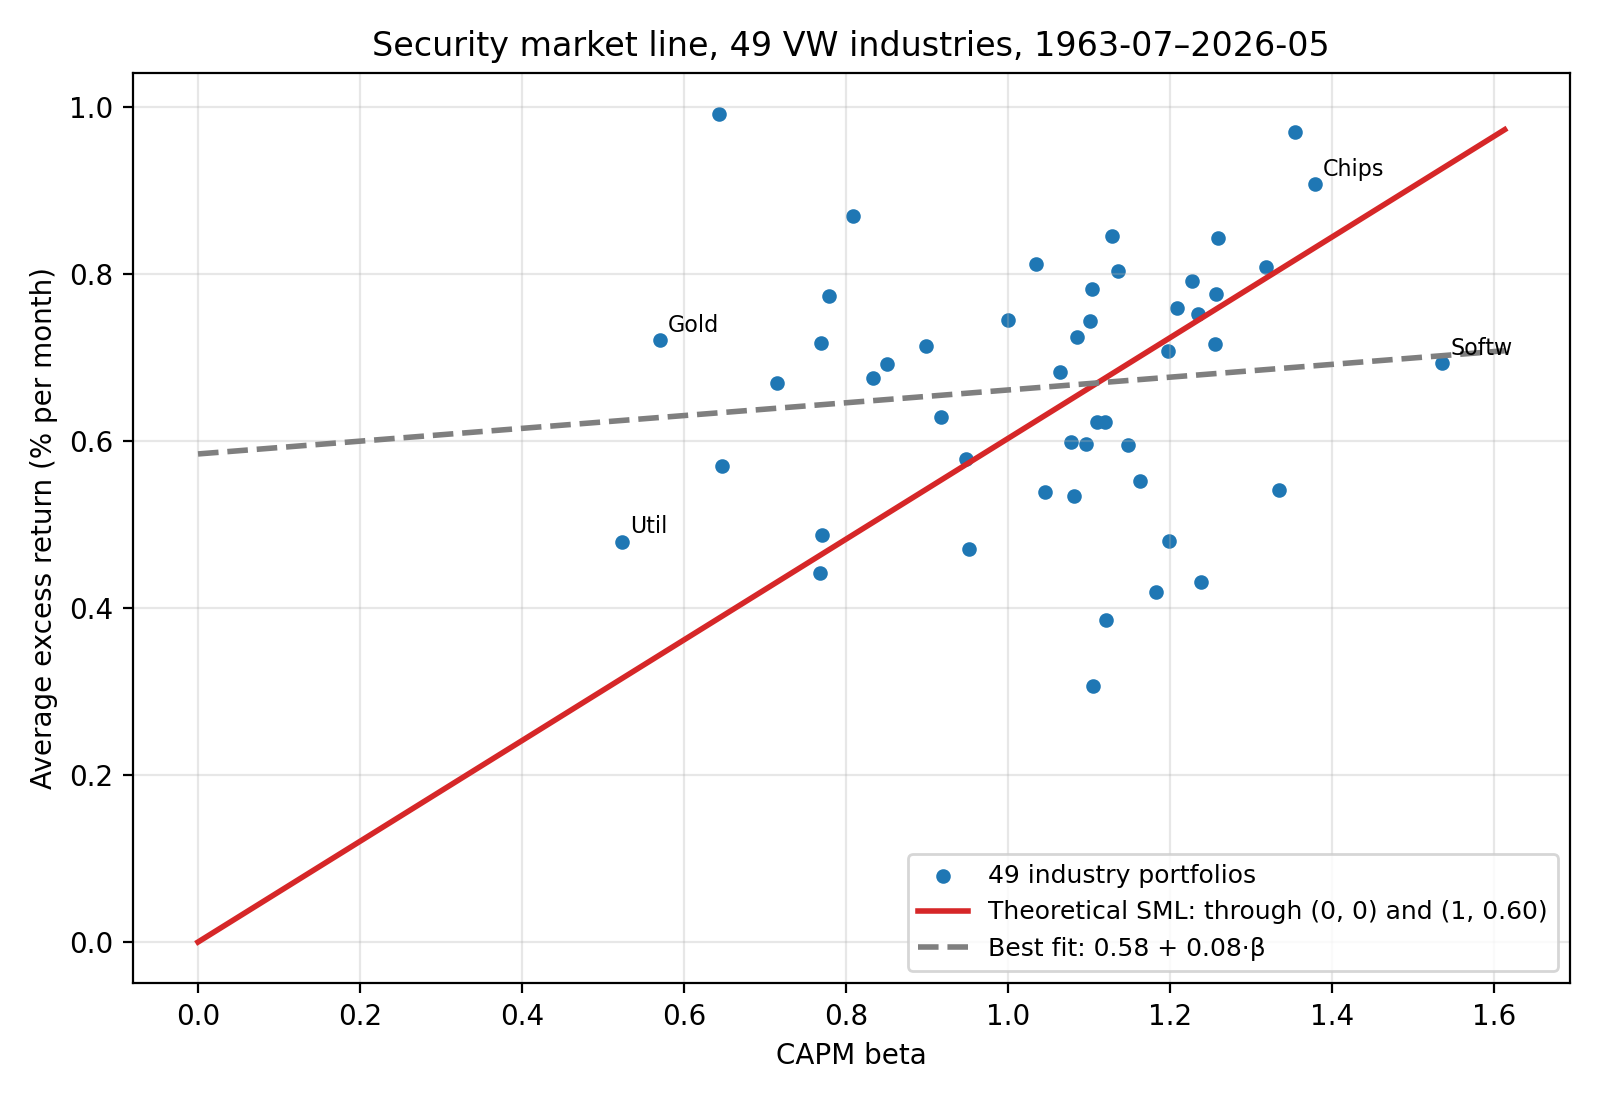
\includegraphics[width=0.8\textwidth]{fig_part2_sml.png}
\caption{Average excess return against CAPM beta for the 49 value-weighted industries, 1963:07--2026:05. The solid red line is the theoretical SML through $(0,0)$ and $(1,\bar r^e_m)$. The dashed grey line is the OLS fit through the 49 points.}
\label{fig:sml}
\end{figure}

\subsection*{(d)}
\begin{itemize}
  \item \textbf{The shape contradicts the CAPM.} Under the CAPM, every industry should sit on a line through the origin whose slope equals the market premium. The data instead form a roughly flat cloud: average beta nearly doubles from the lowest to the highest quintile (Table~\ref{tab:betas}), yet average returns stay between 0.61\% and 0.74\%.
\end{itemize}

\subsection*{(e)}
\begin{itemize}
  \item \textbf{Two known points pin down the SML.} The risk-free asset has $\beta=0$ and zero excess return. The market has $\beta=1$ and an average excess return of $\bar r^e_m=0.60\%$. The SML is the line through $(0,0)$ and $(1,0.60)$, shown in red in Figure~\ref{fig:sml}.
\end{itemize}

\subsection*{(f)}
\begin{itemize}
  \item \textbf{The fitted line is much flatter than theory.} The OLS fit is $\bar r^e_i = 0.58 + 0.08\,\hat\beta_i$. The intercept is well above zero ($t=5.52$), the slope is not significant ($t=0.77$), and $R^2=0.01$. Theory predicts an intercept of 0 and a slope of 0.60.
  \item \textbf{Possible causes.} Leverage constraints push demand toward high-beta assets. Errors in the estimated betas bias the fitted slope toward zero. Beta may also stand in for exposures to other factors that are priced.
  \item \textbf{Implication for asset pricing.} Market beta alone does not explain the cross-section of returns. Either additional factors are needed, or the beta--return relationship is mispriced, leaving a potential opportunity for investors who can borrow.
\end{itemize}

\subsection*{(g)}
\begin{itemize}
  \item \textbf{Investors who cannot borrow buy high-beta assets instead.} Margin limits, leverage bans on mutual funds and pensions, and benchmarking with tracking-error limits all stop investors from levering up low-beta assets. To reach their target return they buy high-beta stocks, which raises those prices and lowers future returns (Black, 1972; Frazzini and Pedersen, 2014).
  \item \textbf{Short-sale limits make it worse.} Arbitrageurs find it hard to short the overpriced high-beta assets, so the mispricing persists.
\end{itemize}

\subsection*{(h)}
\begin{itemize}
  \item \textbf{Go long low-beta and short high-beta.} If the CAPM is the true model, low-beta assets have positive alpha and high-beta assets negative alpha. Lever the low-beta leg and de-lever the high-beta leg so each has a beta of 1. The position is market-neutral with a positive expected return, which is essentially how BAB is built. It is available only to investors who can borrow.
\end{itemize}


\section{Part III: Using the BAB Factor}

\subsection*{(a)--(b)}
\begin{itemize}
  \item \textbf{Pass 1.} For each industry, a full-sample OLS regression of its excess return on RMRF, SMB, HML, UMD and BAB gives the factor loadings $\hat b_i, \hat s_i, \hat h_i, \hat u_i, \hat d_i$.
  \item \textbf{Pass 2.} Each month $t$, a cross-sectional OLS regression of industry excess returns on the estimated loadings (with an intercept) gives the monthly premia $\hat\lambda_t$.
  \item \textbf{Inference.} Each reported premium is the time-series average of $\hat\lambda_t$. Its standard error is $\mathrm{SD}(\hat\lambda_t)/\sqrt{T}$, the $t$-statistic is the ratio of the two, and the $p$-value is two-sided.
\end{itemize}

\subsection*{(c)}
\begin{table}[H]
\centering
\caption{Fama--MacBeth estimates, 49 value-weighted industries, 1963:07--2026:05 ($T=755$). Premia in \% per month. Average cross-sectional $R^2=0.27$.}
\label{tab:fm_bab}
\begin{tabular}{lccccc}
\toprule
 & Premium & Std.\ dev. & Std.\ err. & $t$-stat & $p$-value \\
\midrule
Intercept & 0.414 & 8.39 & 0.305 & 1.35 & 0.18 \\
RMRF      & 0.307 & 9.55 & 0.347 & 0.88 & 0.38 \\
SMB       & $-0.118$ & 4.88 & 0.178 & $-0.66$ & 0.51 \\
HML       & $-0.137$ & 5.43 & 0.198 & $-0.69$ & 0.49 \\
UMD       & 0.314 & 11.66 & 0.424 & 0.74 & 0.46 \\
BAB       & 0.054 & 7.80 & 0.284 & 0.19 & 0.85 \\
\bottomrule
\end{tabular}
\end{table}

\subsection*{(d)}
\begin{itemize}
  \item \textbf{BAB exposure does not explain differences in expected returns across industries.} The estimated BAB premium is 0.05\% ($t=0.19$), far below BAB's own average return of 0.74\%. For a traded factor these should roughly match.
  \item \textbf{This is not surprising.} Industry portfolios vary little in their BAB loadings, and those loadings are strongly negatively correlated with the market loading ($\rho=-0.61$), so the two effects are hard to separate in the cross-section. BAB is also mainly a mispricing story (leverage constraints) rather than compensation for a separate risk, so there is no strong reason to expect industries' BAB loadings to price their returns.
\end{itemize}

\subsection*{(e)}
\begin{itemize}
  \item \textbf{The market premium is too low.} At 0.31\%, it is insignificant and about half the 0.60\% market average. Together with the positive intercept (0.41\%), this shows the flat SML from Part II persists even after controlling for four other factors.
  \item \textbf{No factor is significant.} SMB and HML even come out with negative premia, although both factors have positive average returns. This points to collinear loadings and weak identification on 49 industries rather than real evidence on the factors. UMD loadings barely differ across industries (cross-industry SD of 0.09), which explains why UMD has the largest standard error despite its high average return.
  \item \textbf{The $R^2$ overstates the model's fit.} An average cross-sectional $R^2$ of 0.27 with five loadings on 49 portfolios is not demanding, and the adjusted figure is lower.
  \item \textbf{The $t$-statistics are, if anything, too high.} They ignore the estimation error in the first-pass loadings. A Shanken correction would widen the standard errors further.
\end{itemize}

% Problem Set 7 -- Part IV (revised, concise, for \input after partB.tex).
% Required packages in the group preamble: booktabs, float, caption.
% Full supporting calculations: ps7_partC.py,
% table_part4_results.csv and ps7_partC_llm_log.md.

\section{Part IV: Comparing Quality}

\noindent\textbf{Method.} We use the same two-pass Fama--MacBeth procedure as Part III,
with 49 value-weighted industries, monthly excess returns in percentage points,
and a common sample of July 1963--May 2026 ($T=755$). The first pass estimates
industry factor loadings; the second pass estimates monthly cross-sectional
premia. Reported standard errors are the time-series standard deviation of
monthly premia divided by $\sqrt{T}$, as in Part III. We independently reproduced
the Part III BAB results and checked the calculations using a separate implementation.

\subsection*{(a)--(b) Replacing BAB with QMJ and RMW}
The first specification adds QMJ to RMRF, SMB, HML and UMD; the second substitutes
RMW for QMJ. We re-estimate the first-pass loadings for each specification.

\begin{table}[H]
\centering
\caption{QMJ specification. Fama--MacBeth estimates, $T=755$; premia, standard deviations and standard errors in \% per month. Average monthly cross-sectional $R^2=0.300$.}
\label{tab:ps7_qmj}
\begin{tabular}{lrrrrr}
\toprule
Factor & Premium & SD & SE & $t$-stat & $p$-value \\
\midrule
Intercept & 0.492 & 7.395 & 0.269 & 1.83 & 0.068 \\
RMRF & 0.243 & 8.486 & 0.309 & 0.79 & 0.432 \\
SMB & $-0.120$ & 4.411 & 0.161 & $-0.75$ & 0.456 \\
HML & $-0.124$ & 4.467 & 0.163 & $-0.76$ & 0.446 \\
UMD & 0.315 & 11.556 & 0.421 & 0.75 & 0.454 \\
QMJ & $-0.044$ & 4.171 & 0.152 & $-0.29$ & 0.773 \\
\bottomrule
\end{tabular}
\end{table}

\begin{table}[H]
\centering
\caption{RMW specification; units as in Table~\ref{tab:ps7_qmj}. Average monthly cross-sectional $R^2=0.286$.}
\label{tab:ps7_rmw}
\begin{tabular}{lrrrrr}
\toprule
Factor & Premium & SD & SE & $t$-stat & $p$-value \\
\midrule
Intercept & 0.428 & 7.294 & 0.265 & 1.61 & 0.107 \\
RMRF & 0.291 & 8.481 & 0.309 & 0.94 & 0.346 \\
SMB & $-0.118$ & 4.927 & 0.179 & $-0.66$ & 0.509 \\
HML & $-0.128$ & 4.766 & 0.173 & $-0.74$ & 0.460 \\
UMD & 0.314 & 11.496 & 0.418 & 0.75 & 0.453 \\
RMW & 0.032 & 4.794 & 0.174 & 0.18 & 0.854 \\
\bottomrule
\end{tabular}
\end{table}

\noindent QMJ's estimated premium is $-0.044\%$ per month ($t=-0.29$), while RMW's
is $0.032\%$ ($t=0.18$). These estimates are economically small (about
$-4.4$ and $+3.2$ basis points per month) relative to their standard errors.
Neither is significantly different from zero, despite their positive realized
factor means (0.323\% and 0.246\%, respectively). QMJ's estimated premium
falls significantly short of its factor mean (gap $t=-2.93$); for RMW the gap
is not significant ($t=-1.39$). The market-beta premium is also insignificant
in both specifications.

\subsection*{(c) Including BAB, QMJ and RMW simultaneously}
The joint specification includes all three quality-related factors alongside
RMRF, SMB, HML and UMD.

\begin{table}[H]
\centering
\caption{Joint Fama--MacBeth specification; units as in Table~\ref{tab:ps7_qmj}. Average monthly cross-sectional $R^2=0.352$.}
\label{tab:ps7_joint}
\begin{tabular}{lrrrrr}
\toprule
Factor & Premium & SD & SE & $t$-stat & $p$-value \\
\midrule
Intercept & 0.515 & 8.472 & 0.308 & 1.67 & 0.095 \\
RMRF & 0.215 & 9.360 & 0.341 & 0.63 & 0.528 \\
SMB & $-0.318$ & 4.378 & 0.159 & $-1.99$ & 0.047 \\
HML & $-0.216$ & 4.960 & 0.181 & $-1.20$ & 0.232 \\
UMD & 0.353 & 11.739 & 0.427 & 0.83 & 0.409 \\
BAB & $-0.166$ & 8.550 & 0.311 & $-0.53$ & 0.595 \\
QMJ & $-0.077$ & 4.184 & 0.152 & $-0.51$ & 0.612 \\
RMW & 0.213 & 4.096 & 0.149 & 1.43 & 0.153 \\
\bottomrule
\end{tabular}
\end{table}

\noindent None of the three quality-factor premia is significant at 5\%, individually
or jointly (Wald $\chi^2_3=4.37$, $p=0.22$). SMB is the only factor premium
significant at 5\% ($-0.318\%$, $t=-1.99$, $p=0.047$), but its sign
contrasts with its positive sample mean, so this isolated result warrants caution. The RMRF premium moves from $0.307\%$ in the
Part III BAB model to $0.243\%$ with QMJ, $0.291\%$ with RMW, and $0.215\%$
in the joint model. All four estimates are insignificant and numerically below
the market-factor mean of $0.603\%$, but none is statistically distinguishable
from that mean. For comparison, RMRF is $0.279\%$ ($t=0.94$) without any
quality factor and $0.326\%$ ($t=1.07$) with QMJ+RMW; adding BAB to the
latter changes it to $0.215\%$ ($t=0.63$). The direction of the shift is
not stable across specifications.

\subsection*{(d) How does QMJ affect our interpretation of BAB?}
QMJ does not make us view BAB as simply a mislabeled quality premium: BAB was
not priced in Part III ($0.054\%$, $t=0.19$) and remains insignificant in the
joint test ($-0.166\%$, $t=-0.53$). QMJ itself has no significant
industry-level premium, so there is no evidence that it explains away BAB in
cross-sectional pricing. In separate \emph{time-series} spanning tests, BAB
retains positive alpha with both other quality factors ($0.355\%$,
Newey--West $t=2.72$, six lags). Its QMJ loading falls from approximately
$0.375$ with QMJ alone to $0.036$ when RMW is also included, consistent with
much of BAB's overlap with QMJ running through profitability. This does not
establish a causal mechanism. BAB still primarily reflects beta and leverage
constraints, whereas QMJ includes profitability, growth and safety; factor
spanning is distinct from pricing the 49 industries.

\subsection*{(e) Which measure of quality is better? Are they the same?}
Consistent with Part I, we rank Novy--Marx gross profitability first for
its simplicity and transparency. Among the three factors tested here, RMW
is our preferred measure of fundamental quality because its construction
and interpretation are more straightforward. QMJ combines profitability,
growth and safety but requires more discretion, while BAB primarily reflects
beta and leverage constraints. This ranking concerns measurement, not
whether RMW prices industry returns better than QMJ.

QMJ and RMW have correlated factor returns ($\rho=0.69$),
whereas BAB's correlations with QMJ and RMW are lower (0.21 and 0.32).
In time-series spanning regressions controlling for the four base factors and
other quality factors, QMJ retains positive alpha (0.294\%, $t=5.13$); RMW's
conditional alpha is negative ($-0.133\%$, $t=-2.02$). These results show
partial overlap and asymmetric \emph{factor-return} relationships, not that
QMJ definitively subsumes RMW in cross-sectional expected-return pricing.

\subsection*{(f) Which explains the cross-section of expected returns?}
Of the separate models, QMJ has the highest average \emph{monthly} cross-sectional
$R^2$ (0.300; BAB 0.274, RMW 0.286), versus 0.227 for the four-factor
benchmark; the QMJ+RMW model reaches 0.323 and the joint model 0.352.
However, monthly $R^2$ measures fit to realized monthly returns, and adding
regressors tends to increase it. Regressing \emph{average} industry returns on
loadings gives adjusted $R^2=0.042$ for the four-factor benchmark, 0.037 for
QMJ alone and 0.116 for the joint model (0.118 for QMJ+RMW). QMJ has slightly
better raw monthly fit among the separate specifications, but no individual
quality factor has a significant pricing premium; the larger joint fit is
not compelling evidence of incremental expected-return pricing power.

\subsection*{AI integration: conceptual probe and critical audit}
\noindent\textbf{Prior hypothesis.} From the separate and joint Fama--MacBeth
results, we found no significant quality premium. Before querying the LLM,
we hypothesized that QMJ and RMW share a profitability component while BAB
mainly captures a distinct low-beta mechanism. The spanning analysis had
already been computed when the hypothesis was recorded, so it is not an
out-of-sample prediction.

\noindent\textbf{LLM question and response.} We asked Claude Sonnet the assigned
question: ``BAB, QMJ, and RMW are all sometimes called `quality' factors. Are
they capturing the same underlying effect, or distinct ones? How would you
test whether one subsumes the others?'' It distinguished the factors and
proposed spanning regressions, conditional sorts and factor decompositions.
The full response is recorded in \texttt{ps7\_partC\_llm\_log.md}.

\noindent\textbf{Audit.} (i) The LLM proposed genuine redundancy tests, including
spanning regressions and conditional sorts. It did not explicitly propose the
joint cross-sectional premium test in (c), and it blurred GRS with
Huberman--Kandel spanning conditions.
(ii) It correctly identified BAB as a beta/leverage-constraint strategy rather
than fundamental quality and did not treat the three factors as interchangeable.
It also noted that QMJ's safety component includes beta, so some conceptual
overlap with BAB is built into its definition. But it incorrectly listed payout
as a fourth QMJ pillar (the assigned three are profitability, growth and safety).
(iii) The LLM anticipated partial overlap and suggested that QMJ and BAB
could retain residual spanning alpha; those were useful testable hypotheses,
not assertions about industry-level premia. Its phrase that BAB and RMW
are ``correlated less strongly'' was ambiguous about the comparator: in our
sample BAB--RMW is 0.32, versus BAB--QMJ 0.21 and QMJ--RMW 0.69.
The LLM did not predict the Fama--MacBeth results. QMJ and RMW have opposite-
signed, insignificant separate premia ($-0.044\%$ and $0.032\%$). Adding BAB
raises RMRF from $0.279\%$ ($t=0.94$) to $0.307\%$ ($t=0.88$) in the basic
model but lowers it from $0.326\%$ ($t=1.07$) with QMJ+RMW to $0.215\%$
($t=0.63$) jointly; none is significant. Monthly cross-sectional $R^2$ rises
from 0.227 for the four-factor benchmark to 0.300 with QMJ, 0.286 with RMW
and 0.352 jointly. These fits do not establish a significant premium or prove
that the underlying economic mechanisms are identical.

% Problem Set 7 -- Part V. Converted verbatim from part I &V/PS7_PartI&V.docx.

\section{Part V: Concluding}

\subsection*{Question 1}
I propose a time-series state-dependence test of whether BAB, QMJ, and RMW reflect different economic mechanisms. Using monthly returns, I would regress each factor's next-month return on lagged state variables (a funding-liquidity measure such as the TED spread, VIX, and the Baker--Wurgler sentiment index), controlling for RMRF, SMB, HML, and UMD, with Newey--West standard errors. To separate prediction from contemporaneous effects, I would also regress same-month factor returns on changes in funding conditions. Frazzini and Pedersen's leverage-constraint theory implies BAB should lose when funding tightens contemporaneously, while tighter constraints should raise its expected subsequent returns. QMJ may instead gain through flight to quality, as the lecture shows, and RMW serves as a benchmark for profitability-based quality. Distinct coefficient patterns would support different mechanisms, while similar patterns would suggest a common channel. State dependence cannot distinguish risk compensation from mispricing or establish causality, but it shows which factors respond to financing frictions or sentiment.

\subsection*{Question 2}
\paragraph{Proposed Factor: Margin Resilience Minus Fragility (MRF)}

\paragraph{1. Factor Concept}
I propose Margin Resilience Minus Fragility (MRF), which measures a firm's ability to maintain profitability when input costs rise.

Unlike Novy-Marx's gross profitability and Fama-French's RMW, which measure profitability levels, MRF captures profitability resilience. Two equally profitable firms may differ in pricing power, supplier flexibility, and cost management. Unlike QMJ, which combines profitability, growth, safety, and payout, or BAB, which captures leverage constraints and market beta, MRF focuses specifically on operational resilience.

\paragraph{2. Measurement}
I would measure resilience through the sensitivity of gross margins to industry input-cost changes.

First, calculate quarterly gross margin:
\[
\mathrm{GM} = \frac{\mathrm{Revenue} - \mathrm{COGS}}{\mathrm{Revenue}}
\]
Then estimate a rolling regression over the previous 20 quarters:
\[
\Delta\mathrm{GM}_{i,t} = \alpha_i + \beta_i\Delta P_{j,t} + \gamma_i g_{i,t} + \varepsilon_{i,t}
\]
Where:
\begin{tight}
  \item $\Delta\mathrm{GM}$: Change in gross margin.
  \item $\Delta P$: Industry input-price growth.
  \item $g$: Firm revenue growth, controlling for demand.
  \item $\beta$: Gross-margin sensitivity to input-cost inflation.
\end{tight}

A higher $\beta$ indicates greater resilience, while a strongly negative coefficient indicates fragility. Data would come from Compustat and BLS producer price indices.

\paragraph{3. Portfolio Construction}
Each quarter, I would rank firms by their estimated $\beta$ within industries, using only publicly available information. The strategy would buy the top 20\% (most resilient) and short the bottom 20\% (most fragile), forming value-weighted, industry-neutral portfolios rebalanced quarterly.
\[
\text{MRF Return} = \text{Return on Resilient Firms} - \text{Return on Fragile Firms}
\]

\paragraph{4. Expected Returns}
I hypothesize that resilient firms could earn higher future risk-adjusted returns because investors may undervalue their ability to sustain earnings during cost shocks, creating potential mispricing.

Alternatively, fragile firms may carry greater exposure to inflation or supply shocks and therefore command higher expected returns as risk compensation, potentially producing a negative MRF premium.

I would test these explanations by examining MRF's alpha after controlling for Fama-French factors, momentum, QMJ, and BAB, and its performance during inflation shocks.


\paragraph{Comment.}
MRF is interesting because it measures a firm's ability to maintain profitability during cost shocks rather than its current profitability level. However, I am not convinced it captures a new dimension of quality. Because changes in gross margin depend partly on the COGS-to-revenue ratio, the signal may overlap with gross profitability and RMW, and it resembles QMJ's safety dimension. Measurement is also a concern: industry PPIs may not reflect firms' actual input costs, and 20 quarters of data could produce noisy coefficients, so I would test whether the estimates are stable over time.

The return prediction is not convincing as stated. The proposal offers both a mispricing story (positive premium) and a risk story (negative premium) without committing to a sign, so it cannot be falsified. The risk story would also make MRF an inflation beta rather than a quality factor. I would pre-specify the sign and test alpha against FF5, momentum, QMJ and BAB.


\end{document}
